\documentclass[a4paper,12pt]{book}

%Template per documenti e tesi

\usepackage{titlesec}
\titlespacing*{\section}{0pt}{0.0\baselineskip}{\baselineskip}

\usepackage[utf8]{inputenc}
\usepackage[italian]{babel}
\usepackage{float}
\usepackage{graphicx}
\usepackage[left=2.5cm,right=2.5cm,top=3cm,bottom=3cm]{geometry}
\usepackage{hyperref}
\usepackage{setspace}
\usepackage{shapepar}
\usepackage{listings}
\usepackage[table,xcdraw]{xcolor}
\usepackage{fonttable}
\usepackage{amssymb}
\usepackage{amsmath}
%\usepackage{enumerate}
%\usepackage{enumitem}
\usepackage{fontawesome}

\usepackage{color} %red, green, blue, yellow, cyan, magenta, black, white
\definecolor{mygreen}{RGB}{28,172,0} % color values Red, Green, Blue
\definecolor{mylilas}{RGB}{170,55,241}

\colorlet{punct}{red!60!black}
\definecolor{background}{HTML}{EEEEEE}
\definecolor{delim}{RGB}{20,105,176}
\colorlet{numb}{magenta!60!black}
\definecolor{dkgreen}{rgb}{0,0.6,0}
\definecolor{gray}{rgb}{0.5,0.5,0.5}
\definecolor{mauve}{rgb}{0.58,0,0.82}

\lstdefinelanguage{mySQL}{%
	language     = SQL,
	morekeywords = {STDDEV, FLOOR, MATERIALIZED, IF, ROUND},
}

\lstset{frame=tb,
	language=Java,
	%aboveskip=3mm,
	%belowskip=3mm,
	showstringspaces=false,
	columns=flexible,
	basicstyle=\small\ttfamily,
	numbers=none,
	numberstyle=\scriptsize,
	keywordstyle=\color{blue},
	commentstyle=\color{dkgreen},
	stringstyle=\color{mauve},
	breaklines=true,
	breakatwhitespace=true,
	tabsize=3
}


\lstdefinelanguage{json}{
	basicstyle=\small\ttfamily,
	numbers=left,
	numberstyle=\scriptsize,
	stepnumber=1,
	numbersep=8pt,
	showstringspaces=false,
	breaklines=true,
	frame=lines,
	backgroundcolor=\color{background},
}

\hypersetup{
	colorlinks=false,
	linktoc=all, %both sections and subsections linked
}

\usepackage[hyperref,backend=bibtex,backref,backrefstyle=none,sorting=none]{biblatex}
\addbibresource{references.bib}
\usepackage{fancyhdr}

\newcommand{\makelogo}{%
	\centering
	\textsc{Università degli Studi di Napoli Federico II}
	\\[.4cm]
	\textsc{Dipartimento di Ingegneria Elettrica e Tecnologie dell'Informazione}
	\\[1.1cm]
	
\includegraphics[width=0.7\textwidth]{./figures/logo_blu.png}\\[1.1cm]
	\textsc{Corso di Laurea Magistrale in Informatica\\A.A. 2017-18}
	\\[2.5cm]
	\textbf{Progetto Basi di Dati II Modulo B}
	\vfill
	%\end{par}
	\centering
	\begin{par}
		\begin{tabular}{lllll}
			& \textbf{Autori} &                        &  &  \\
			\textbf{Bizzarri Flavio} & \textbf{}       & \textbf{Cuomo Daniele} &  &  \\
			\textbf{N97000281}       & \textbf{}       & \textbf{N97000270}     &  &  \\
			&                 &                        &  & 
		\end{tabular}
	
	\end{par}
	%\par
}

\fancyhead{}
\fancyhead[LO,LE]{\slshape\nouppercase\leftmark}
\cfoot{\thepage}

\pagestyle{fancy}

\DefineBibliographyStrings{italian}{%
	bibliography = {Riferimenti},
}

\begin{document}

	
	\onehalfspacing
	%\doublespacing use in case of emergency
	\author{F. Bizzarri, D. Cuomo}
	\title{Progetto Finale Basi di Dati II}
	
	{\frontmatter
		\let\cleardoublepage\clearpage{\makelogo}
		\thispagestyle{empty}
		
		\chapter*{\centering {\normalsize Sommario}}
Si vuole realizzare un data warehouse destinato all’analisi di dati riguardanti misurazioni effettuate su veicoli da parte dell’Istituto Motori di Napoli.
Le misurazioni effettuate si concentrano sull'emissione di particelle di inquinanti in tratti stradali misti e presentano anche la componente spaziale rappresentata dalle coordinate GPS dei rilevamenti.
Il DW realizzato ed esposto in questo documento è di tipo ROLAP, implementato con PostgreSQL, il quale fornisce sia tutte caratteristiche necessarie al data warehousing sia un’estensione spaziale.
		
		\tableofcontents
		
		\thispagestyle{empty}
		\mainmatter
	}
	
	
	\let\cleardoublepage\clearpage{		
		%\include{./chapters/intro}
		\chapter{Progettazione}
In questa capitolo sono esposte le scelte progettuali usate come linee guida per l'implementazione di una base di dati orientata al data warehousing.
\section{Interrogazioni}
Nella tabella \ref{table:query} sono riportate le query che si intende sottoporre al sistema. Ogni query ha ad essa associata un numero identificativo ed una descrizione dell'analisi che si intende effettuare.
\begin{table}[H]
	\centering
\begin{tabular}{cll}
	\rowcolor[HTML]{333333} 
	{\color[HTML]{FFFFFF} \#} & {\color[HTML]{FFFFFF} Query}                                                                                       & {\color[HTML]{FFFFFF} Obiettivo}                                                                                                                                                                                                                   \\
	1                         & \begin{tabular}[c]{@{}l@{}}Impatto ambientale medio in corse\\ da 5 km (CO2 e NOx, massa)\end{tabular}             & \begin{tabular}[c]{@{}l@{}}Pensata per analizzare varianti della\\ stessa interrogazione su diversi livelli\\ di granularità\end{tabular}                                                                                                          \\
	\rowcolor[HTML]{C0C0C0} 
	2                         & \begin{tabular}[c]{@{}l@{}}Consumo medio per intervalli di\\ velocità prefissati, su tutto il dataset\end{tabular} & \begin{tabular}[c]{@{}l@{}}Utile all'implementazione e l'analisi\\ di viste materializzate che\\ raggruppano i dati secondo delle \\ fasce di velocità. Le fasce scelte, \\ espresse in km/h, sono le seguenti:\\ 0-50, 50-90, 90-130\end{tabular} \\
	3                         & \begin{tabular}[c]{@{}l@{}}Efficienza dell'auto per intervalli\\ di RPM (rotazioni per minuto)\end{tabular}        & \begin{tabular}[c]{@{}l@{}}Altra interessante interrogazione\\ creata allo scopo di sfruttare le\\ viste materializzate. Il dataset \\ fornisce tutti i parametri \\ necessari al calcolo dell'efficienza, \\ o rendimento istantaneo\end{tabular} \\
	\rowcolor[HTML]{C0C0C0} 
	4                         & \begin{tabular}[c]{@{}l@{}}Per ogni test, media di NOx,\\ CO2, Potenza e Velocità\end{tabular}                     & \begin{tabular}[c]{@{}l@{}}Quest'interrogazione serve a\\ valutare le prestazioni ottenute\\ dall'esecuzione su di un \\ partizionamento verticale con le\\ colonne sparse tra più tabelle\end{tabular}                                            \\
	5                         & \begin{tabular}[c]{@{}l@{}}Media e deviazione standard\\ delle temperature\end{tabular}                            & \begin{tabular}[c]{@{}l@{}}Quest'interrogazione serve a \\ valutare le prestazioni ottenute\\ dall'esecuzione con le colonne \\ concentrate su di un unica\\ tabella restituita da un\\ partizionamento verticale\end{tabular}                    
\end{tabular}
\label{table:query}
\end{table}
Le query sopra riportate hanno guidato lo sviluppo del sistema in ogni sua fase e hanno permesso di sperimentare differenti tecniche di implementazione di un sistema ROLAP.
Una definizione formale delle stesse in linguaggio SQL sarà presentata più avanti nel corso di questo documento.
\section{Diagrammi}
Di seguito è riportato il diagramma UML che rappresenta lo schema dei fatti implementato secondo il modello relazionale ROLAP.
\begin{figure}[H]
	\centering
	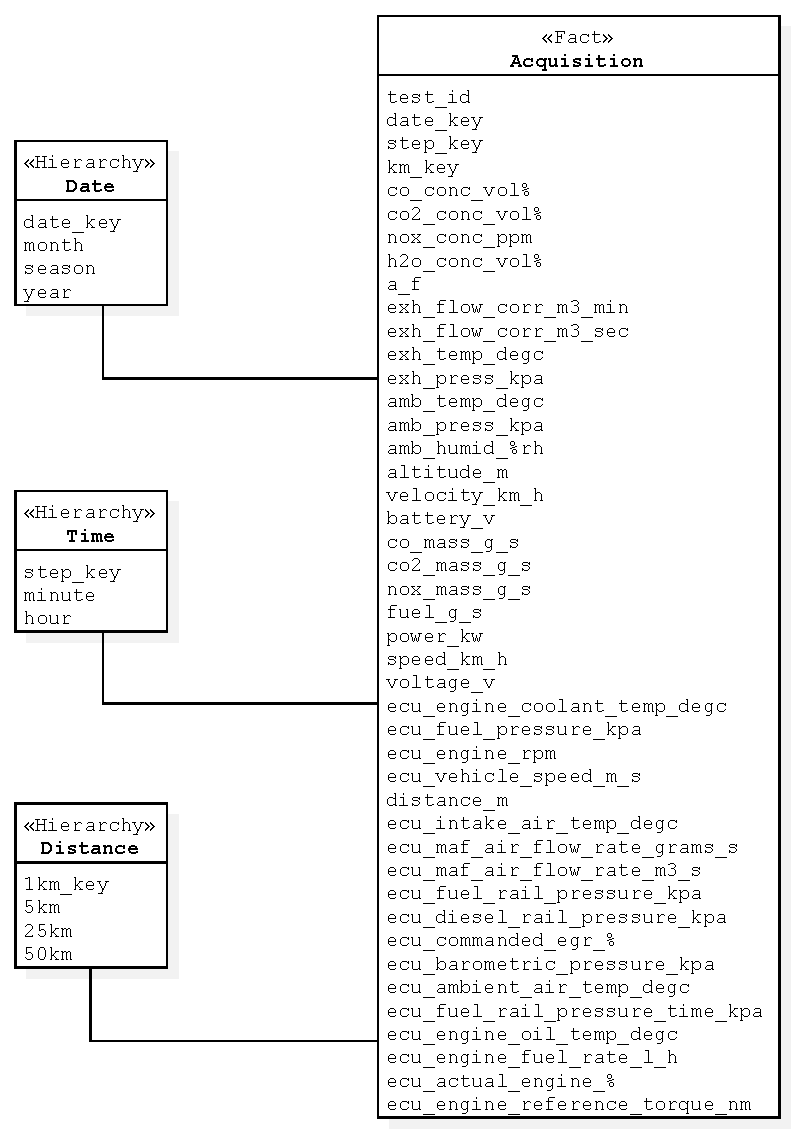
\includegraphics[scale=0.56]{figures/class_fact_scheme}
	\caption{Diagaramma UML schema dei fatti}
	\label{fig:ofm}
\end{figure}
È stata inoltre progettata e implementata una variante dello schema proposto che sfrutta la tecnica del partizionamento verticale ovvero la possibilità di dividere la tabella dei fatti in più tabelle, ognuna delle quali rappresenta una particolare sfaccettatura del \textit{fatto}. Il partizionamento viene solitamente adoperato per agevolare quelle interrogazioni che riguardano solo una particolare area di interesse. Per poter applicare questa tecnica è necessario aggiungere una chiave tra le tabelle al fine di poterle ricongiungere per analizzare il dato nella sua completezza.
\begin{figure}[H]
	\centering
	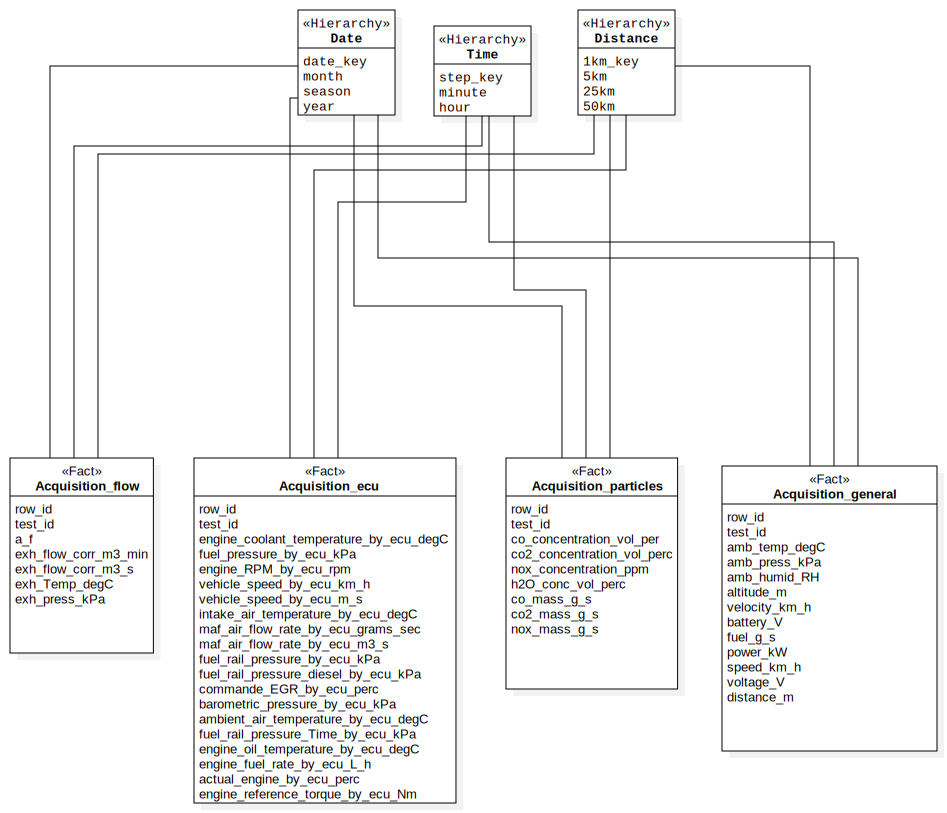
\includegraphics[scale=0.6]{figures/class_fact_scheme_part} %TODO cambiare diagaramma
	\caption{Diagramma UML schema dei fatti partizionato verticalmente}
	\label{fig:ofm}
\end{figure}
\newpage
\section{ETL}
Al fine di avere un numero rilevante di dati per l'analisi dei tempi è stato implementato un meccanismo di duplicazione dei file.
La procedura ETL sviluppata si compone di differenti passaggi descritti nella seguente tabella.
\begin{table}[H]
	\centering
	\begin{tabular}{clll}
		\rowcolor[HTML]{333333} 
		{\color[HTML]{FFFFFF} \#}	& {\color[HTML]{FFFFFF} Passaggio}	& {\color[HTML]{FFFFFF} Descrizione}	& {\color[HTML]{FFFFFF} Implementazione}
		\\
		1							& \begin{tabular}[c]{@{}l@{}}Trasformazione dei file\\ XLSX in formato CSV\end{tabular}
																		& \begin{tabular}[c]{@{}l@{}}Eliminazione delle righe contenenti \\dati inconsistenti\\Calcolo dei campi formula\\Creazione di una data fittizia \\Creazione di un test\_id\\Salvataggio in formato CSV\end{tabular}
																									            & \begin{tabular}[c]{@{}l@{}}Java\end{tabular}
		\\
		\rowcolor[HTML]{C0C0C0} 
		2                         & \begin{tabular}[c]{@{}l@{}}Importazione dei dati in\\ tabella provvisoria\end{tabular} 
																		& \begin{tabular}[c]{@{}l@{}}Viene sfruttata il comando copy\\ del DBMS per importare i dati\\ in maniera efficiente\end{tabular}
																												 & \begin{tabular}[c]{@{}l@{}}PostgreSQL\end{tabular} 
		\\
		3                         & \begin{tabular}[c]{@{}l@{}}Shutdown degli indici\end{tabular}        
																		& \begin{tabular}[c]{@{}l@{}}\end{tabular}
																												 & \begin{tabular}[c]{@{}l@{}}PostgreSQL\end{tabular}
		\\
		\rowcolor[HTML]{C0C0C0} 
		4                         & \begin{tabular}[c]{@{}l@{}}Aggiornamento dello schema\end{tabular}                     
																		& \begin{tabular}[c]{@{}l@{}}Aggiornamento delle dimensioni\\Aggiornamento tabella dei fatti\end{tabular}            
																												 & \begin{tabular}[c]{@{}l@{}}PostgreSQL\end{tabular}	                      
		\\	
		5                         & \begin{tabular}[c]{@{}l@{}}Riattivazione degli indici\end{tabular}             
																		& \begin{tabular}[c]{@{}l@{}}\end{tabular}  
																												 & \begin{tabular}[c]{@{}l@{}}PostgreSQL\end{tabular}    
		\\
		\rowcolor[HTML]{C0C0C0} 
		6                         & \begin{tabular}[c]{@{}l@{}}Aggiornamento viste\end{tabular}                     
																		& \begin{tabular}[c]{@{}l@{}}\end{tabular}            
																												 & \begin{tabular}[c]{@{}l@{}}PostgreSQL\end{tabular}	
	\end{tabular}
\end{table}
Per righe inconsistenti si intendono tutte quelle righe ove per valori indicanti volumi e/o concentrazioni vi sono valori negativi; inoltre viene dedotta la distanza percorsa ove mancante sfruttando la distanza percorsa e le velocità istantanee rilevate negli istanti precedenti.


\section{Viste Materializzate}
Sono state create le seguenti viste materializzate al fine di implementare efficacemente le query 2 e 3.
\\
Il primo frammento dichiara una vista contenente per ogni corsa (\textit{test\_id}) il carburante consumato suddiviso per fasce di velocità.
\begin{lstlisting}[language=SQL]
CREATE MATERIALIZED VIEW IF NOT EXISTS fuel_compare_speed AS
SELECT t1.id, t1.fuel_litres as consumo_litri_meno_di_50km_h, t2.fuel_litres as consumo_litri_meno_di_90km_h, t3.fuel_litres as consumo_litri_meno_di_130km_h
FROM
(SELECT test_id as id, round(SUM((fuel_g_s)/1000)::numeric/0.8,2) AS fuel_litres, round(AVG(velocity_km_h)::numeric,1) as average_speed_km_h
FROM acquisition_fact
where speed_km_h <=50
GROUP BY test_id) t1
JOIN (
SELECT test_id as id, round(SUM((fuel_g_s)/1000)::numeric/0.8,2) AS fuel_litres, round(AVG(velocity_km_h)::numeric,1) as average_speed_km_h
FROM acquisition_fact
WHERE speed_km_h >=50 and speed_km_h<=90
GROUP BY test_id
) t2
ON t1.id=t2.id
JOIN (
SELECT test_id as id , round(SUM((fuel_g_s)/1000)::numeric/0.8,2) AS fuel_litres, round(AVG(velocity_km_h)::numeric,1) as average_speed_km_h
FROM acquisition_fact
WHERE speed_km_h >=90
GROUP BY test_id
)t3
ON t1.id=t3.id;
\end{lstlisting}

L'estratto a seguire serve a calcolare una vista materializzata riportante l'efficienza dell'auto nelle diverse corse. I risultati sono stati distribuiti su 3 fasce di rotazioni per minuto (RPM).
\begin{lstlisting}[language=SQL]
CREATE MATERIALIZED VIEW IF NOT EXISTS efficiency_compare_rpm AS
SELECT t1.id,  round((t1.rendimento*100)::numeric, 2) as efficiency_perc_max2000rpm, round((t2.rendimento*100)::numeric,2) as efficiency_perc_max3000rpm, round((t3.rendimento*100)::numeric,2) as efficiency_perc_over3000rpm
FROM
(SELECT test_id as id, avg(power_kw)/ (avg(fuel_g_s)/1000 * 458000) as rendimento
FROM acquisition_fact
WHERE engine_RPM_by_ecu_rpm <2000
GROUP BY test_id) t1
JOIN (
SELECT test_id as id, avg(power_kw)/ (avg(fuel_g_s)/1000 * 458000) as rendimento
FROM acquisition_fact
WHERE engine_RPM_by_ecu_rpm >=2000 and engine_RPM_by_ecu_rpm <=3000
GROUP BY test_id
) t2
ON  t1.id=t2.id
JOIN (
SELECT  test_id as id, avg(power_kw)/( avg(fuel_g_s)/1000 * 458000) as rendimento
FROM acquisition_fact
WHERE engine_RPM_by_ecu_rpm >=3000
GROUP BY test_id
)t3
ON t1.id=t3.id;
\end{lstlisting}
		\chapter{Analisi}
In questo capitolo sono riportati i risultati e i tempi ottenuti per ogni fase: dalle procedure ETL all'esecuzione delle query.

\section{ETL}
\subsection{Trasformazione in CSV}
In questa sezione copriremo un'analisi dei tempi ottenuti nella fase che permette, a partire dai dati originali, di ottenere un file in formato CSV contenente i dati ripuliti da inconsistenze e in un formato adatto ad essere importato nel Datawarehouse.
In particolare nella fase di puliza, a partire dal file XSLX, si estraggono unicamente i record dove non appaiono valori negativi per quantità intrinsecamente positive (concentrazione, volume, ecc.); per i record ove manca il valore "relative" e/o la distanza percorsa si procede ad un calcolo a partire dall'ultima rilevazione valida estratta. Inoltre tutte le righe che presentano una chiara assenza di dati (70\% delle colonne) vengono scartate. Infine, durante la fase di trasformazione, per ogni file viene generata una data e un test\_id e per separare la parte intera da quella decimale si sostituisce la virgola con il punto.\\
I dati ottenuti si riferiscono ad una media aritmetica ottenuta testando 200 file ($\sim$1 milione di righe) generati a partire dal file originario fornito dall'Istituto Motori di Napoli.

\begin{table}[H]
	\centering
\begin{tabular}{ccccc}
	\rowcolor[HTML]{333333} 
	{\color[HTML]{FFFFFF}Righe XSLX}  
	& 
	{\color[HTML]{FFFFFF}Righe CSV}
	&
	{\color[HTML]{FFFFFF}Righe perse}
	&
	{\color[HTML]{FFFFFF}Peso file XSLX}
	&                                 
	{\color[HTML]{FFFFFF}Peso file CSV}\\
	\begin{tabular}[c]{@{}l@{}}5764\end{tabular}             
	& \begin{tabular}[c]{@{}l@{}}5706\end{tabular} 
	& \begin{tabular}[c]{@{}l@{}}1\%\end{tabular}  
	& \begin{tabular}[c]{@{}l@{}}2.138KB\end{tabular}  
	& \begin{tabular}[c]{@{}l@{}}2.283KB\end{tabular}   
\end{tabular}
\end{table}

\begin{table}[H]
	\centering
	\begin{tabular}{ccc}
		\rowcolor[HTML]{333333} 
	{\color[HTML]{FFFFFF}Fase di pulizia}
	&
	{\color[HTML]{FFFFFF}Fase di trasformazione}
	&
	{\color[HTML]{FFFFFF}Tempo totale}\\
	\begin{tabular}[c]{@{}l@{}}3.04s\end{tabular}             
	& \begin{tabular}[c]{@{}l@{}}0,05s\end{tabular} 
	& \begin{tabular}[c]{@{}l@{}}3,05s\end{tabular}
\end{tabular}
\end{table}

Questa fase mette in luce la buona qualità dei dati forniti dall'istituto: ci si aspetta in media di perdere pochissimi dati a causa di inconsistenze. Per quanto riguarda invece le dimensioni si nota come il formato Comma-separated values sia leggermente meno efficiente nella compressione rispetto al formato proprietario di Microsoft$^{\tiny{\textregistered}}$ ma al tempo stesso permetta una più veloce elaborazione.

\subsection{Import in tabella temporanea}
Al fine di importare i file CSV nella tabella dei fatti ci si appoggia ad una tabella temporanea al fine di agevolare le operazioni successive. Questa tabella viene troncata alla fine della procedura. L'import sfrutta la funzione \textit{COPY} messa a disposizione dal DBMS PostgreSQL.

\begin{table}[H]
	\centering
	\begin{tabular}{ccc}
		\rowcolor[HTML]{333333} 
		{\color[HTML]{FFFFFF}Numero file}
		&
		{\color[HTML]{FFFFFF}Numero righe}
		&
		{\color[HTML]{FFFFFF}Tempo}\\
		\begin{tabular}[c]{@{}l@{}}1\end{tabular}             
		& \begin{tabular}[c]{@{}l@{}}5706\end{tabular} 
		& \begin{tabular}[c]{@{}l@{}}214ms\end{tabular}\\
		\rowcolor[HTML]{C0C0C0}
		\begin{tabular}[c]{@{}l@{}}50\end{tabular}             
		& \begin{tabular}[c]{@{}l@{}}285.300\end{tabular} 
		& \begin{tabular}[c]{@{}l@{}}8,428s\end{tabular}\\
		\begin{tabular}[c]{@{}l@{}}100\end{tabular}             
		& \begin{tabular}[c]{@{}l@{}}570.600\end{tabular} 
		& \begin{tabular}[c]{@{}l@{}}16.522s\end{tabular}
	\end{tabular}
\caption{I dati si riferiscono ad una media di 5 esecuzioni}
\end{table}	
I risultati mostrano la bontà della funzione \textit{COPY} che sfruttando un inserimento batch di 1000 righe per volta riesce ad abbattere in modo consistente i tempi.

\subsection{Import nello schema}
In questa fase i dati, precedentemente inseriti in una tabella temporanea, vengono travasati nello schema proposto dopo aver disabilitato tutti gli indici. Le prove effettuate prendono in considerazione diverse dimensioni della tabella dei fatti oltre al caso in cui lo schema risulti partizionato.
\begin{table}[H]
	\centering
	\begin{tabular}{cccc}
		\rowcolor[HTML]{333333} 
		{\color[HTML]{FFFFFF}Dimensione tab. fatti}
		&
		{\color[HTML]{FFFFFF}Numero righe importate}
		&
		{\color[HTML]{FFFFFF}Partizionamento}
		&
		{\color[HTML]{FFFFFF}Tempo}\\
		\begin{tabular}[c]{@{}l@{}}0\end{tabular}             
		& \begin{tabular}[c]{@{}l@{}}285.300\end{tabular} 
		& \begin{tabular}[c]{@{}l@{}}No\end{tabular}
		& \begin{tabular}[c]{@{}l@{}}3,925s\end{tabular}\\
		\rowcolor[HTML]{C0C0C0}
		\begin{tabular}[c]{@{}l@{}}0\end{tabular}             
		& \begin{tabular}[c]{@{}l@{}}285.300\end{tabular} 
		& \begin{tabular}[c]{@{}l@{}}Si\end{tabular}
		& \begin{tabular}[c]{@{}l@{}}7,753s\end{tabular}\\
		\begin{tabular}[c]{@{}l@{}}570.600\end{tabular}             
		& \begin{tabular}[c]{@{}l@{}}285.300\end{tabular} 
		& \begin{tabular}[c]{@{}l@{}}No\end{tabular}
		& \begin{tabular}[c]{@{}l@{}}3,730s\end{tabular}\\
		\rowcolor[HTML]{C0C0C0}
		\begin{tabular}[c]{@{}l@{}}570.600\end{tabular}             
		& \begin{tabular}[c]{@{}l@{}}285.300\end{tabular} 
		& \begin{tabular}[c]{@{}l@{}}Si\end{tabular}
		& \begin{tabular}[c]{@{}l@{}}7,404s\end{tabular}\\
		\begin{tabular}[c]{@{}l@{}}1.141.200\end{tabular}             
		& \begin{tabular}[c]{@{}l@{}}285.300\end{tabular} 
		& \begin{tabular}[c]{@{}l@{}}No\end{tabular}
		& \begin{tabular}[c]{@{}l@{}}4,535s\end{tabular}\\
		\rowcolor[HTML]{C0C0C0}
		\begin{tabular}[c]{@{}l@{}}1.141.200\end{tabular}             
		& \begin{tabular}[c]{@{}l@{}}285.300\end{tabular} 
		& \begin{tabular}[c]{@{}l@{}}Si\end{tabular}
		& \begin{tabular}[c]{@{}l@{}}8,572s\end{tabular}
		
	\end{tabular}
	\caption{I dati si riferiscono ad una media di 5 esecuzioni}
\end{table}	
Dalla tabella emerge come il partizionamento comporti quasi un raddoppio del tempo necessario all'inserimento: ciò è dovuto al dover spalmare un singolo record della tabella temporanea su 4 differenti tabelle. Questo slow-down è risolvibile pensando a 4 inserimenti in parallelo: infatti le 4 tabelle, anche se logicamente collegate, durante l'inserimento non necessitano di condividere alcuna informazione.

\subsection{Aggiornamento degli indici}
In questa fase vengono riattivati gli indici delle chiavi tra tabella dei fatti e dimensioni. Questi indici sono assolutamente necessari per velocizzare le query ma possono essere disabilitati durante la fase di update dello schema.
\begin{table}[H]
	\centering
	\begin{tabular}{ccc}
		\rowcolor[HTML]{333333} 
		{\color[HTML]{FFFFFF}Dimensione tab. fatti}
		&
		{\color[HTML]{FFFFFF}Partizionamento}
		&
		{\color[HTML]{FFFFFF}Tempo}\\
		\begin{tabular}[c]{@{}l@{}}285.300\end{tabular}              
		& \begin{tabular}[c]{@{}l@{}}No\end{tabular}
		& \begin{tabular}[c]{@{}l@{}}2,530s\end{tabular}\\
		\rowcolor[HTML]{C0C0C0}
		\begin{tabular}[c]{@{}l@{}}285.300\end{tabular}              
		& \begin{tabular}[c]{@{}l@{}}Si\end{tabular}
		& \begin{tabular}[c]{@{}l@{}}11,534s\end{tabular}\\	\begin{tabular}[c]{@{}l@{}}570.600\end{tabular}              
		& \begin{tabular}[c]{@{}l@{}}No\end{tabular}
		& \begin{tabular}[c]{@{}l@{}}6,194s\end{tabular}\\
		\rowcolor[HTML]{C0C0C0}
		\begin{tabular}[c]{@{}l@{}}570.600\end{tabular}              
		& \begin{tabular}[c]{@{}l@{}}Si\end{tabular}
		& \begin{tabular}[c]{@{}l@{}}24,715s\end{tabular}\\
		\begin{tabular}[c]{@{}l@{}}1.141.200\end{tabular}              
		& \begin{tabular}[c]{@{}l@{}}No\end{tabular}
		& \begin{tabular}[c]{@{}l@{}}16,903s\end{tabular}\\
		\rowcolor[HTML]{C0C0C0}
		\begin{tabular}[c]{@{}l@{}}1.141.200\end{tabular}              
		& \begin{tabular}[c]{@{}l@{}}Si\end{tabular}
		& \begin{tabular}[c]{@{}l@{}}67,469s\end{tabular}\\
		\begin{tabular}[c]{@{}l@{}}1.426.500\end{tabular}              
		& \begin{tabular}[c]{@{}l@{}}No\end{tabular}
		& \begin{tabular}[c]{@{}l@{}}24,141s\end{tabular}\\
		\rowcolor[HTML]{C0C0C0}
		\begin{tabular}[c]{@{}l@{}}1.426.500\end{tabular}              
		& \begin{tabular}[c]{@{}l@{}}Si\end{tabular}
		& \begin{tabular}[c]{@{}l@{}}98,218s\end{tabular}
		
	\end{tabular}
	\caption{I dati si riferiscono ad una media di 5 esecuzioni}
\end{table}	
Dai dati sopra mostrati emerge ancora una volta come l'introduzione di un partizionamento verticale comporti un notevole rallentamento. In particolare la forbice tra i tempi registrati aumenta all'aumentare della dimensione dei fatti. Ciò induce a pensare attentamente all'introduzione di un partizionamento in fase di progettazione valutando il rapporto costo/benefici.

\subsection{Aggiornamento delle viste materializzate}
A valle dell'inserimento dei nuovi record si rende necessario l'aggiornamento delle viste materializzate utilizzate per velocizzare le query 3 e 4.
\begin{table}[H]
	\centering
	\begin{tabular}{ccc}
		\rowcolor[HTML]{333333} 
		{\color[HTML]{FFFFFF}Dimensione tab. fatti}
		&
		{\color[HTML]{FFFFFF}Efficiency\_compare\_rpm\_mv}
		&
		{\color[HTML]{FFFFFF}Fuel\_compare\_speed\_mv}\\
		\begin{tabular}[c]{@{}l@{}}285.300\end{tabular}              
		& \begin{tabular}[c]{@{}l@{}}0,307s\end{tabular}
		& \begin{tabular}[c]{@{}l@{}}0,238s\end{tabular}\\
		\rowcolor[HTML]{C0C0C0}
		\begin{tabular}[c]{@{}l@{}}570.600\end{tabular}              
		& \begin{tabular}[c]{@{}l@{}}0,983s\end{tabular}
		& \begin{tabular}[c]{@{}l@{}}0,898s\end{tabular}\\
	    \begin{tabular}[c]{@{}l@{}}1.141.200\end{tabular}              
		& \begin{tabular}[c]{@{}l@{}}2,464s\end{tabular}
		& \begin{tabular}[c]{@{}l@{}}2,173s\end{tabular}\\
		\rowcolor[HTML]{C0C0C0}
		\begin{tabular}[c]{@{}l@{}}1.426.500\end{tabular}              
		& \begin{tabular}[c]{@{}l@{}}3,004s\end{tabular}
		& \begin{tabular}[c]{@{}l@{}}2,863s\end{tabular}\\
		
	\end{tabular}
	\caption{I dati si riferiscono ad una media di 5 esecuzioni}
\end{table}
I tempi osservati mostrano come un raddoppio del numero di record comporti un più che raddoppio del tempo necessario all'aggiornamento delle viste. Notevole è infatti l'incremento di tempo per materializzare la vista con 1.141.200 record: 2.5 volte quello necessario per materializzare la vista con la metà dei record. 
\section{Analisi Performance Query}
In questa sezione verranno analizzate le query implementate nelle differenti implementazioni e presentati gli snippet di codice SQL

\subsection{Query I}
\subsubsection{Impatto ambientale medio in corse da 5 km}
%\begin{lstlisting}[language=SQL]
%SELECT J.km_5, AVG(J.sum_co2) AS avg_co2, AVG(J.sum_nox) AS %avg_nox
%FROM (
%	SELECT H.km_5, SUM(F.co2_mass_g_s) AS sum_co2, SUM(F.nox_mass_g_s) AS sum_nox
%	FROM acquisition_fact F, distance_hierarchy H
%	WHERE (F.km_key::INT / 1000) = H.km_key
%	GROUP BY F.test_id, H.km_5) J
%GROUP BY J.km_5
%\end{lstlisting} COSA CAMBIA?

A seguire sono proposte due diverse formulazioni della stessa interrogazione. Il primo estratto chiede al sistema di recuperare l'appartenenza ad una certa tratta (di 5 km) dalla tabella \textit{distance\_hierarchy}. Nella seconda forma la tratta viene calcolata, eseguendo quindi un'operazione di roll-up implicito.
\subsubsection{Roll-up esplicito}
\begin{lstlisting}[language=SQL]
SELECT F.test_id, H.km_5, AVG(F.co2_mass_g_s), AVG(F.nox_mass_g_s)
FROM acquisition_fact F INNER JOIN distance_hierarchy H
	ON (F.km_key = H.km_key)
GROUP BY F.test_id, H.km_5
\end{lstlisting}

\subsubsection{Roll-up implicito}
\begin{lstlisting}[language=SQL]
SELECT F.test_id, FLOOR(F.km_key/5), AVG(F.co2_mass_g_s), AVG(F.nox_mass_g_s)
FROM acquisition_fact F
GROUP BY F.test_id, FLOOR(F.km_key/5)
\end{lstlisting}

\subsubsection{Esito}
L'estrazione dei tempi di esecuzione delle due query può fornire una misura di utilità di una dimensione. In questo caso è interessante notare come un \textit{fatto} possa essere ricondotto alla sua dimensione di appartenenza attraverso un calcolo richiedente 2 operazioni elementari.

\subsection{Query C}
\subsubsection{Consumo medio per intervalli di velocità prefissati}
L'utilizzo della vista materializzata permette di abbattere i tempi di esecuzione della query fino a un trecentesimo: in questo modo il costo di aggiornamento della vista viene immediatamente ammortizzato.
\begin{table}[H]
	\centering
	\begin{tabular}{ccc}
		\rowcolor[HTML]{333333} 
		{\color[HTML]{FFFFFF}Dimensione tab. fatti}
		&
		{\color[HTML]{FFFFFF}Senza vista}
		&
		{\color[HTML]{FFFFFF}Con vista}\\
		\begin{tabular}[c]{@{}l@{}}570.600\end{tabular}              
		& \begin{tabular}[c]{@{}l@{}}0,905s\end{tabular}
		& \begin{tabular}[c]{@{}l@{}}0,020\end{tabular}\\
		\rowcolor[HTML]{C0C0C0}
		\begin{tabular}[c]{@{}l@{}}1.141.200\end{tabular}              
		& \begin{tabular}[c]{@{}l@{}}2,286s\end{tabular}
		& \begin{tabular}[c]{@{}l@{}}0,026s\end{tabular}\\
		\begin{tabular}[c]{@{}l@{}}1.426.500\end{tabular}              
		& \begin{tabular}[c]{@{}l@{}}2,925s\end{tabular}
		& \begin{tabular}[c]{@{}l@{}}0.028s\end{tabular}\\
	\end{tabular}
\caption{Test effettuati su schema non partizionato}
\end{table}
\begin{lstlisting}[language=SQL]
SELECT *
FROM fuel_compare_speed_mv;
\end{lstlisting}
\begin{lstlisting}[language=SQL]
SELECT t1.id, t1.fuel_litres as consumo_litri_meno_di_50km_h, t2.fuel_litres as consumo_litri_meno_di_90km_h, t3.fuel_litres as consumo_litri_meno_di_130km_h
FROM
(SELECT test_id as id, round(SUM((fuel_g_s)/1000)::numeric/0.8,2) AS fuel_litres, round(AVG(velocity_km_h)::numeric,1) as average_speed_km_h
FROM acquisition_fact
where speed_km_h <=50
GROUP BY test_id) t1
JOIN (
SELECT test_id as id, round(SUM((fuel_g_s)/1000)::numeric/0.8,2) AS fuel_litres, round(AVG(velocity_km_h)::numeric,1) as average_speed_km_h
FROM acquisition_fact
where speed_km_h >=50 and speed_km_h<=90
GROUP BY test_id
) t2
ON t1.id=t2.id
JOIN (
SELECT test_id as id , round(SUM((fuel_g_s)/1000)::numeric/0.8,2) AS fuel_litres, round(AVG(velocity_km_h)::numeric,1) as average_speed_km_h
FROM acquisition_fact
where speed_km_h >=90
GROUP BY test_id
)t3
ON t1.id=t3.id;
\end{lstlisting}

\subsection{Query E}
\subsubsection{Efficienza dell'auto per intervalli di RPM}
Si conferma quanto osservato nel caso della \textit{query 2}: utilizzare una vista materializzata permette di abbattere i tempi di esecuzione della query e il costo del refresh risulta ampiamente ammortizzato.
\begin{table}[H]
	\centering
	\begin{tabular}{ccc}
		\rowcolor[HTML]{333333} 
		{\color[HTML]{FFFFFF}Dimensione tab. fatti}
		&
		{\color[HTML]{FFFFFF}Senza vista}
		&
		{\color[HTML]{FFFFFF}Con vista}\\
		\begin{tabular}[c]{@{}l@{}}570.600\end{tabular}              
		& \begin{tabular}[c]{@{}l@{}}0,937s\end{tabular}
		& \begin{tabular}[c]{@{}l@{}}0,018s\end{tabular}\\
		\rowcolor[HTML]{C0C0C0}
		\begin{tabular}[c]{@{}l@{}}1.141.200\end{tabular}              
		& \begin{tabular}[c]{@{}l@{}}2,182s\end{tabular}
		& \begin{tabular}[c]{@{}l@{}}0,028s\end{tabular}\\
		\begin{tabular}[c]{@{}l@{}}1.426.500\end{tabular}              
		& \begin{tabular}[c]{@{}l@{}}2,892s\end{tabular}
		& \begin{tabular}[c]{@{}l@{}}0,030s\end{tabular}\\
		
	\end{tabular}
\caption{Test effettuati su schema non partizionato}
\end{table}
\begin{lstlisting}[language=SQL]
select *
from efficiency_compare_rpm_mv;
\end{lstlisting}
\begin{lstlisting}[language=SQL]
SELECT t1.id,  round((t1.rendimento*100)::numeric, 2) as efficiency_perc_max2000rpm, round((t2.rendimento*100)::numeric,2) as efficiency_perc_max3000rpm, round((t3.rendimento*100)::numeric,2) as efficiency_perc_over3000rpm
FROM
(SELECT test_id as id, avg(power_kw)/ (avg(fuel_g_s)/1000 * 458000) as rendimento
FROM acquisition_fact
where engine_RPM_by_ecu_rpm <2000
GROUP BY test_id) t1
JOIN (
SELECT test_id as id, avg(power_kw)/ (avg(fuel_g_s)/1000 * 458000) as rendimento
FROM acquisition_fact
where engine_RPM_by_ecu_rpm >=2000 and engine_RPM_by_ecu_rpm <=3000
GROUP BY test_id
) t2
ON  t1.id=t2.id
JOIN (
SELECT  test_id as id, avg(power_kw)/( avg(fuel_g_s)/1000 * 458000) as rendimento
FROM acquisition_fact
where engine_RPM_by_ecu_rpm >=3000
GROUP BY test_id
)t3
ON t1.id=t3.id;
\end{lstlisting}

\subsection{Query M}
\subsubsection{Per ogni test, media di NOx, CO2, Potenza e Velocità}
TODO. Qui la query dovrebbe essere più veloce senza il partizionamento.
\begin{table}[H]
	\centering
	\begin{tabular}{ccc}
		\rowcolor[HTML]{333333} 
		{\color[HTML]{FFFFFF}Dimensione tab. fatti}
		&
		{\color[HTML]{FFFFFF}Partizionamento}
		&
		{\color[HTML]{FFFFFF}Tempo}\\
		\begin{tabular}[c]{@{}l@{}}570.600\end{tabular}              
		& \begin{tabular}[c]{@{}l@{}}No\end{tabular}
		& \begin{tabular}[c]{@{}l@{}}6,194s\end{tabular}\\
		\rowcolor[HTML]{C0C0C0}
		\begin{tabular}[c]{@{}l@{}}570.600\end{tabular}              
		& \begin{tabular}[c]{@{}l@{}}Si\end{tabular}
		& \begin{tabular}[c]{@{}l@{}}24,715s\end{tabular}\\
		\begin{tabular}[c]{@{}l@{}}1.141.200\end{tabular}              
		& \begin{tabular}[c]{@{}l@{}}No\end{tabular}
		& \begin{tabular}[c]{@{}l@{}}16,903s\end{tabular}\\
		\rowcolor[HTML]{C0C0C0}
		\begin{tabular}[c]{@{}l@{}}1.141.200\end{tabular}              
		& \begin{tabular}[c]{@{}l@{}}Si\end{tabular}
		& \begin{tabular}[c]{@{}l@{}}67,469s\end{tabular}\\
		\begin{tabular}[c]{@{}l@{}}1.426.500\end{tabular}              
		& \begin{tabular}[c]{@{}l@{}}No\end{tabular}
		& \begin{tabular}[c]{@{}l@{}}24,141s\end{tabular}\\
		\rowcolor[HTML]{C0C0C0}
		\begin{tabular}[c]{@{}l@{}}1.426.500\end{tabular}              
		& \begin{tabular}[c]{@{}l@{}}Si\end{tabular}
		& \begin{tabular}[c]{@{}l@{}}98,218s\end{tabular}
		
	\end{tabular}
\end{table}	
\begin{lstlisting}[language=SQL]
NO Partizionamento
\end{lstlisting}
\begin{lstlisting}[language=SQL]
SI partizionamento
\end{lstlisting}


\subsection{Query T}
\subsubsection{Media e deviazione standard delle temperature}
TODO. Qui la query dovrebbe essere più veloce con il partizionamento.
\begin{table}[H]
	\centering
	\begin{tabular}{ccc}
		\rowcolor[HTML]{333333} 
		{\color[HTML]{FFFFFF}Dimensione tab. fatti}
		&
		{\color[HTML]{FFFFFF}Partizionamento}
		&
		{\color[HTML]{FFFFFF}Tempo}\\
		\begin{tabular}[c]{@{}l@{}}570.600\end{tabular}              
		& \begin{tabular}[c]{@{}l@{}}No\end{tabular}
		& \begin{tabular}[c]{@{}l@{}}6,194s\end{tabular}\\
		\rowcolor[HTML]{C0C0C0}
		\begin{tabular}[c]{@{}l@{}}570.600\end{tabular}              
		& \begin{tabular}[c]{@{}l@{}}Si\end{tabular}
		& \begin{tabular}[c]{@{}l@{}}24,715s\end{tabular}\\
		\begin{tabular}[c]{@{}l@{}}1.141.200\end{tabular}              
		& \begin{tabular}[c]{@{}l@{}}No\end{tabular}
		& \begin{tabular}[c]{@{}l@{}}16,903s\end{tabular}\\
		\rowcolor[HTML]{C0C0C0}
		\begin{tabular}[c]{@{}l@{}}1.141.200\end{tabular}              
		& \begin{tabular}[c]{@{}l@{}}Si\end{tabular}
		& \begin{tabular}[c]{@{}l@{}}67,469s\end{tabular}\\
		\begin{tabular}[c]{@{}l@{}}1.426.500\end{tabular}              
		& \begin{tabular}[c]{@{}l@{}}No\end{tabular}
		& \begin{tabular}[c]{@{}l@{}}24,141s\end{tabular}\\
		\rowcolor[HTML]{C0C0C0}
		\begin{tabular}[c]{@{}l@{}}1.426.500\end{tabular}              
		& \begin{tabular}[c]{@{}l@{}}Si\end{tabular}
		& \begin{tabular}[c]{@{}l@{}}98,218s\end{tabular}
		
	\end{tabular}
\end{table}	
\begin{lstlisting}[language=SQL]
NO Partizionamento
\end{lstlisting}
\begin{lstlisting}[language=SQL]
SI partizionamento
\end{lstlisting}



		\chapter{Conclusioni}
I risultati ottenuti sono chiaramente legati all'architettura hardware e software utilizzata per l'esecuzione delle procedure. Durante l'intero progetto è stata utilizzata una piattaforma con le seguenti specifiche:
\begin{itemize}
	\item Xiaomi Notebook Air 13
	\item Intel Core i7
	\item SSD da 256GB
	\item RAM da 8GB
	\item Windows 10
\end{itemize}
I tempi sono necessariamente soggetti a limiti fisici e rumori dovuti a:
\begin{enumerate}
	\item Capacità hardware del calcolatore
	\item Scheduling del sistema operativo.
	\item Parametri di configurazione del DBMS.
\end{enumerate}
Per ammortizzare la perturbazione, le fasi di cronometraggio prevedono l'acquisizione di più campioni dello stesso tipo, dai quali si è poi ricavata la media. I valori ottenuti vanno inoltre scalati rispetto alla dimensione del dataset. A tal proposito si è simulata una cardinalità massiccia di acquisizioni (circa 1.5 milioni).\\
A valle dell’analisi condotta si è arrivati alle seguenti riflessioni:
%- Aumentare la quantità di memoria principale a disposizione per le operazioni di raggruppamento, ordinamento e join può sensibilmente migliorare l’esecuzione di alcune query, permettendo l’utilizzo di operazioni completamente in-memory.

\begin{itemize}
	\item Quando una gerarchia coincide con scalare un'unità di misura ci si può imbattere in allocazioni massicce di informazioni ridondanti, senza un gadagno netto in termini temporali. In questo scenario si può quindi optare per operazioni di raggruppamento su espressioni	calcolabili sui fatti, invece che utilizzare l’implementazione tradizionale che prevede una tabella separata per ogni gerarchia e utilizzo di join, che possono appesantire notevolmente il calcolo.
	\item L’utilizzo della vista materializzata ha mostrato, come previsto, un vantaggio notevole, con un rallentamento accettabile della fase di ETL di aggiornamento delle viste.
	\item Il partizionamento non ha mostrato evidenti miglioramenti che ne giustifichino l’utilizzo. Infatti, si è registrato un peggioramento netto della fase di ETL e delle query che prevedono la ricostruzione del fatto. Tuttavia, se ci si trova in un contesto in cui il numero di interrogazioni circoscritte a singole partizioni e significativo, tale tecnica può portare benefici interessanti.
\end{itemize}
		\appendix
		\chapter{Sorgenti Java}
\subsubsection{Main.java}
\lstinputlisting{./sources/java/Main.java}
\subsubsection{Multiplier.java}
\lstinputlisting{./sources/java/Multiplier.java}
\subsubsection{Cleaner.java}
\lstinputlisting{./sources/java/etl/Cleaner.java}
\subsubsection{Transformer.java}
\lstinputlisting{./sources/java/etl/Transformer.java}
		\chapter{Sorgenti SQL}
	}
		
	\backmatter
	%\printbibliography[title=Riferimenti,heading=bibintoc]
	
	%\printglossaries
	%\listoffigures
	%\listoftables
	
	%\let\cleardoublepage\clearpage{
	%	\include{./ringraziamenti/thanks}
	%	\thispagestyle{empty}
	%}
\end{document}